	

	\subsection*{1.}
	
	\subsubsection*{a.	$C(5) = 5^3 - 18 \times 5^2 + 750 \times 5 + 200 = 3625 $ euros.}
	
	\subsubsection*{b.}
	Le coût moyen de fabrication d’un millier d’objets lorsqu’on fabrique 5 000 objets est donc :
	\[
	\dfrac{3625}{5} = 725 \, \text{euros}.
	\]
	
	\subsection*{2.}
	
	Le coût moyen \(CM(q)\) de fabrication de \(q\) milliers d’objets, exprimé en euros, est donné par l’expression :
	
	\[
	CM(q) = \dfrac{C(q)}{q} = q^2 - 18q + 750 + \dfrac{200}{q}.
	\]
	
	\subsubsection*{a.}
		On a sur l’intervalle \([1 ; 20]\),
	\[
	C'_M(q) = 2q - 18 - \dfrac{200}{q^2} = \dfrac{2q^3 - 18q^2 - 200}{q^2}.
	\]
	
	Or
\begin{align*}
	2(q - 10)(q^2 + q + 10) &= (2q - 20)(q^2 + q + 10)\\
	& = 2q^3 + 2q^2 + 20q - 20q^2 - 20q - 200 \\
	&= 2q^3 - 18q^2 - 200
\end{align*}

	
	
	soit le numérateur de \(C'_M(x)\). \\
	Donc, pour tout \(q \in [1 ; 20]\),
	\[
	C'_M(q) = \dfrac{2(q - 10)(q^2 + q + 10)}{q^2}.
	\]
	
	\subsubsection*{b.}
	

	Pour le trinôme \(q^2 + q + 10\), on a \(\Delta = 1 - 40 = -39\) : pas de racines réelles et on sait que le trinôme est positif (signe de 1, coefficient de \(q^2\)).
	
	Comme \(q^2 > 0\) sur \([1 ; 20]\), le signe de \(C'_M(q)\) est celui de \(q - 10\).
	
	Donc sur \([1 ; 10]\), \(C'_M(q) < 0\) :\\
	 La fonction \(C_M\) est décroissante de \(C_M(1) = 1 - 18 + 750 + 200 = 933\)\\
	  à \(C_M(10) = 10^2 - 18 \times 10 + 750 + 20 = 690\).
	
	Sur \([10 ; 20]\), la fonction \(C_M\) est croissante de \(CM(10) = 690\) à \(CM(20) = 20^2 - 18 \times 20 + 750 + 10 = 800\).
	
	\begin{center}
	\begin{tikzpicture}[double distance=2pt]
		\tkzTabInit{$x$/1,$C'_M(x)$/1,$C_M$/3}{$-\infty$,$10$, $+\infty$}
		\tkzTabLine{,-,z,+}
		\tkzTabVar{+/$933$,-/$690$,+/$800$}
	\end{tikzpicture}
\end{center} 
	
	\subsubsection*{c.}
	
	Quel est le coût moyen minimal et pour quelle quantité d’objets est-il obtenu ?
	
	On voit sur le tableau que le coût moyen minimal de 690 est obtenu lorsque l’entreprise fabrique 10 000 objets.
	
